\lstinputlisting[
  firstline=1,
  lastline=33,
  label={code:pi},
  caption={Approximation af pi ved hjælp af python}
]{source/pi.py}
Koden indeholder 2 specielle funktioner:
\begin{itemize}
  \item "computeDerivatives" som beregner de afledte for funktionen f 
  i punktet a, dette sker ved hjælp af python pakken SymPy, herefter returneres disse som en liste af værdier.  
  \item "intergrateTaylor" som beregner værdien af intergralet imellem to endepunkter i et interval
  og returnere værdierne for intergralet ved specifike ordener. 
\end{itemize} 
Når koden køres fåes følgende værdier:
\begin{center}
  \begin{tabular}{ |c|c|c|c|c|c|c| }
    \hline
      Antal led $n$ & 10 & 20 & 50 & 100 & 200 & 500 \\
    \hline
      Approximation & $1.5852$ & $1.5763$ & $1.5723$ & $1.5713$ & $1.5709$ & $1.5708$ \\
    \hline
  \end{tabular}
\end{center}
%\label{tab:approksimationenVsN}
Som det kan ses i tabellen sker der en mindre og mindre ændring i værdien for approksimationen når n bliver større og større
I denne sammenhæng er det også intresant at kigge på fejlen $R$ imellem approksimationen og $\frac{\pi}{2}$:
\begin{figure}[H]
  \centering
  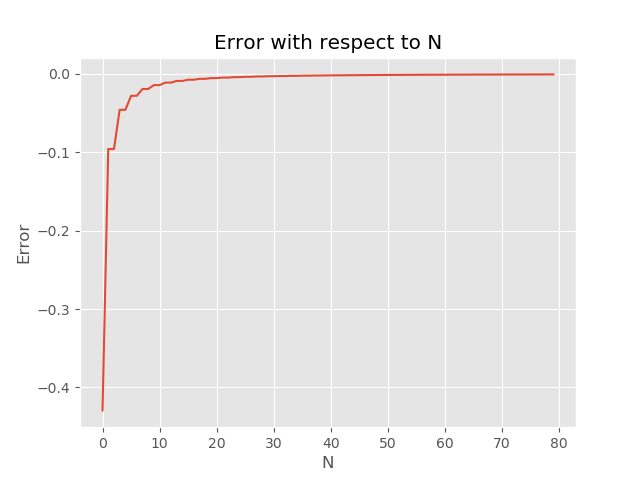
\includegraphics[width=\textwidth]{fig/img/ErrorWithRespectToN.png}
  \caption{Fejl i forhold til antalet af led $n$}
  \label{fig:FejlIForholdTilN}
\end{figure}
Som det kan ses falder fejlen hurtigt i starten når $n$ er lille, men som $n$ vokser flader funktionen ud.